\documentclass[10pt,a4paper]{article}
\usepackage[utf8]{inputenc}
\usepackage[french]{babel}
\usepackage[T1]{fontenc}
\usepackage{amsmath}
\usepackage{amsthm}
\usepackage{amsfonts}
\usepackage{amssymb}
\usepackage{graphicx}
\usepackage{mathrsfs}
\usepackage{url}
\usepackage{color}
\usepackage{listings}
\definecolor{mygreen}{RGB}{28,172,0} % color values Red, Green, Blue
\definecolor{mylilas}{RGB}{170,55,241}
\lstset{
language=R,
basicstyle=\scriptsize\ttfamily,
commentstyle=\ttfamily\color{green},
numbers=left,
numberstyle=\ttfamily\color{black}\footnotesize,
stepnumber=1,
numbersep=5pt,
backgroundcolor=\color{white},
showspaces=false,
showstringspaces=false,
showtabs=false,
frame=single,
tabsize=2,
captionpos=b,
breaklines=true,
breakatwhitespace=false,
keywordstyle=\color{blue},
stringstyle=\color{magenta},
literate=
  {á}{{\'a}}1 {é}{{\'e}}1 {í}{{\'i}}1 {ó}{{\'o}}1 {ú}{{\'u}}1
  {Á}{{\'A}}1 {É}{{\'E}}1 {Í}{{\'I}}1 {Ó}{{\'O}}1 {Ú}{{\'U}}1
  {à}{{\`a}}1 {è}{{\`e}}1 {ì}{{\`i}}1 {ò}{{\`o}}1 {ù}{{\`u}}1
  {À}{{\`A}}1 {È}{{\'E}}1 {Ì}{{\`I}}1 {Ò}{{\`O}}1 {Ù}{{\`U}}1
  {ä}{{\"a}}1 {ë}{{\"e}}1 {ï}{{\"i}}1 {ö}{{\"o}}1 {ü}{{\"u}}1
  {Ä}{{\"A}}1 {Ë}{{\"E}}1 {Ï}{{\"I}}1 {Ö}{{\"O}}1 {Ü}{{\"U}}1
  {â}{{\^a}}1 {ê}{{\^e}}1 {î}{{\^i}}1 {ô}{{\^o}}1 {û}{{\^u}}1
  {Â}{{\^A}}1 {Ê}{{\^E}}1 {Î}{{\^I}}1 {Ô}{{\^O}}1 {Û}{{\^U}}1
  {œ}{{\oe}}1 {Œ}{{\OE}}1 {æ}{{\ae}}1 {Æ}{{\AE}}1 {ß}{{\ss}}1
  {ű}{{\H{u}}}1 {Ű}{{\H{U}}}1 {ő}{{\H{o}}}1 {Ő}{{\H{O}}}1
  {ç}{{\c c}}1 {Ç}{{\c C}}1 {ø}{{\o}}1 {å}{{\r a}}1 {Å}{{\r A}}1
  {€}{{\EUR}}1 {£}{{\pounds}}1
}

\lstset{language=Matlab,%
%basicstyle=\color{red},
breaklines=true,%
morekeywords={matlab2tikz},
keywordstyle=\color{blue},%
morekeywords=[2]{1}, keywordstyle=[2]{\color{black}},
identifierstyle=\color{black},%
stringstyle=\color{mylilas},
commentstyle=\color{mygreen},%
showstringspaces=false,%without this there will be a symbol in the places where there is a space
numbers=left,%
numberstyle={\tiny \color{black}},% size of the numbers
numbersep=9pt, % this defines how far the numbers are from the text
emph=[1]{for,end,break},emphstyle=[1]\color{red}, %some words to emphasise
%emph=[2]{word1,word2}, emphstyle=[2]{style},    
}
\lstset{literate=
{á}{{\'a}}1 {é}{{\'e}}1 {í}{{\'i}}1 {ó}{{\'o}}1 {ú}{{\'u}}1
{Á}{{\'A}}1 {É}{{\'E}}1 {Í}{{\'I}}1 {Ó}{{\'O}}1 {Ú}{{\'U}}1
{à}{{\`a}}1 {è}{{\`e}}1 {ì}{{\`i}}1 {ò}{{\`o}}1 {ù}{{\`u}}1
{À}{{\`A}}1 {È}{{\'E}}1 {Ì}{{\`I}}1 {Ò}{{\`O}}1 {Ù}{{\`U}}1
{ä}{{\"a}}1 {ë}{{\"e}}1 {ï}{{\"i}}1 {ö}{{\"o}}1 {ü}{{\"u}}1
{Ä}{{\"A}}1 {Ë}{{\"E}}1 {Ï}{{\"I}}1 {Ö}{{\"O}}1 {Ü}{{\"U}}1
{â}{{\^a}}1 {ê}{{\^e}}1 {î}{{\^i}}1 {ô}{{\^o}}1 {û}{{\^u}}1
{Â}{{\^A}}1 {Ê}{{\^E}}1 {Î}{{\^I}}1 {Ô}{{\^O}}1 {Û}{{\^U}}1
{œ}{{\oe}}1 {Œ}{{\OE}}1 {æ}{{\ae}}1 {Æ}{{\AE}}1 {ß}{{\ss}}1
{ű}{{\H{u}}}1 {Ű}{{\H{U}}}1 {ő}{{\H{o}}}1 {Ő}{{\H{O}}}1
{ç}{{\c c}}1 {Ç}{{\c C}}1 {ø}{{\o}}1 {å}{{\r a}}1 {Å}{{\r A}}1
{€}{{\euro}}1 {£}{{\pounds}}1 {«}{{\guillemotleft}}1
{»}{{\guillemotright}}1 {ñ}{{\~n}}1 {Ñ}{{\~N}}1 {¿}{{?`}}1
}
\usepackage[french,onelanguage,ruled,lined,linesnumbered]{algorithm2e}
\SetKw{And}{et}
\SetKw{From}{allant de}
\author{\textsc{Adrien WARTELLE} \& \textsc{HABIBALLAH Seddik}}
\title{Rapport de projet OS11}
\date{\today}

\begin{document}
\maketitle
\renewcommand{\contentsname}{Sommaire}
\tableofcontents
\clearpage

\begin{abstract}
Ce projet nous a permis d'étudier 3 heuristiques utilisées pour la résolution (approchée) du problème du voyageur du commerce. Ce problème consiste à trouver un chemin de coût minimal (somme des distances/coûts entre les nœuds du chemin) passant par tous les nœuds d'un graphe. Il s'agit d'un problème NP-difficile, c'est-à-dire que pour trouver la solution optimale, il faut (dans le pire cas) énumérer toute les solutions possibles qui sont au nombre de $n!$, n étant le nombre de nœuds.
Ainsi pour des problèmes de taille moyenne ou grande, comme ici où l'on prendra n=50, il est nécessaire de faire appel à des heuristiques pour avoir un temps d'exécution qui n'"explose" pas\footnote{Autrement dit, que la complexité de l'algorithme de résolution soit polynomial et non exponentiel}. Nous allons donc étudier 3 heuristiques de construction de tour par insertion de nœuds dans un tour non complet : \begin{enumerate}
\item PPI : Plus Proche Insertion
\item PLI : Plus Lointaine Insertion
\item MI : Meilleure Insertion
\end{enumerate}
\end{abstract}

\section{Description des heuristiques}

Les algorithmes par insertion sont des algorithmes qui construisent des tours par 
ajout itératif de nœuds. Chaque heuristique va sélectionner, à chaque itération,
 un nœud d'une manière différente :
 \begin{enumerate}
\item Avec PPI, celui dont la distance au circuit actuel\footnote{qui est la distance minimale
à l'ensemble des nœuds du circuit actuel} est minimale
\item Avec PLI, celui dont la distance au circuit actuel est maximale
\item Avec MI : celui dont le coût d'insertion au circuit actuel est minimale
\end{enumerate}
Après avoir sélectionner le nœud, chacun de ces algorithmes va insérer celui-ci de manière optimale
dans le circuit, c'est-à-dire avec le coût d'insertion minimal. Pour obtenir le coût d'insertion du nouveau après
un nœud candidat dans le circuit, il suffit d'additionner la distance entre le nœud candidat et le nouveau nœud et
la distance du nouveau nœud et le voisin (dans le circuit) du nœud candidat et ensuite de soustraire la distance entre le nœud candidat
et son voisin. On obtient alors la longueur ajouté au circuit si l'on insère le nouveau nœud, ce qui correspond au coût
d'insertion.

On peut alors décrire ces algorithmes comme ceci :

\begin{algorithm}[H]
    \caption{Algorithme PPI : Plus proche insertion}
    
    \tcp{Déclaration et Initialisation}
     $C_{min}$ : Coût minimal d'insertion
     
     $D_{min} \leftarrow +\infty$ : Distance minimale au circuit
     
     $\forall i=1...n,D_{tour}^{i} \leftarrow +\infty$, : Distances des nœuds encore à insérer au circuit
     
     $B$ : Nœud sélectionné à insérer (B pour "Best")
     
     $A \leftarrow 0$ : Nœud d'insertion de coût minimal (A avant B, ou B voisin de A)
     
    \tcp{Recherche du ième point du point à ajouter au chemin actuel}
    \For{$i$ \From $1$ \KwTo $N$}{
    
        \tcp{Réinitialiser le coût et la distance minimales}
        $C_{min} \leftarrow +\infty$
        
        $D_{min} \leftarrow +\infty$
        
        \tcp{Recherche parmi les nœuds qui ne sont pas encore dans le circuit}
        \For{$j$ \From $1$ \KwTo $N$}{
            \If{$j \notin circuit$}{
            Recalculer la distance $D_{tour}^{j}$ du nœud j au circuit en prenant en compte le (i-1)-ème nœud ajouté (nœud $i-1$ du circuit)
            
            Mise à jour de la distance minimale : $D_{min} \leftarrow min(D(B,node(i-1)) ,D(j,node(i-1)))$
           
            
            Mise à jour du meilleur nœud à ajouter : $B \leftarrow arg1min(D(B,node(i-1)) ,D(j,node(i-1)))$  \footnote{node(i-1) est l'index du (i-1)-ème nœud ajouté au circuit et D(,) est la distance entre deux nœuds}
             }
            
	        \If{$j \in circuit$}{
	        Calculer le coût d'ajout $C_{j}$ de B après le nœud j  dans le circuit
	        
	        
	        Mise à jour du coût (minimal) de meilleure insertion : $C_{min} \leftarrow min(C_{A},C_{j})$
	        
	        Mise à jour du nœud (prédécesseur) de meilleure insertion : $A \leftarrow argmin(C_{A},C_{j})$
	        }
        }
        Ajouter le nœud B à la suite du nœud A dans le circuit.
    }
\end{algorithm}

\begin{algorithm}[H]
    \caption{Algorithme PLI : Plus lointaine insertion}
    
    \tcp{Déclaration et Initialisation}
     $C_{min}$ : Coût minimal d'insertion
     
     $D_{max} \leftarrow 0$ : Distance maximale au circuit
     
     $\forall i=1...n,D_{tour}^{i} \leftarrow +\infty$, : Distances des nœuds encore à insérer au circuit
     
     $B$ : Nœud sélectionné à insérer (B pour "Best")
     
     $A \leftarrow 0$ : Nœud d'insertion de coût minimal (A avant B, ou B voisin de A)
     
    \tcp{Recherche du ième point du point à ajouter au chemin actuel}
    \For{$i$ \From $1$ \KwTo $N$}{
    
        \tcp{Réinitialiser le coût et la distance minimales}
        $C_{min} \leftarrow +\infty$
        
        $D_{max} \leftarrow 0$
        
        \tcp{Recherche parmi les nœuds qui ne sont pas encore dans le circuit}
        \For{$j$ \From $1$ \KwTo $N$}{
            \If{$j \notin circuit$}{
            Recalculer la distance $D_{tour}^{j}$ du nœud j au circuit en prenant en compte le (i-1)-ème nœud ajouté (nœud $i-1$ du circuit)
            
            Mise à jour de la distance maximale: $D_{max} \leftarrow max(D(B,node(i-1)) ,D(j,node(i-1)))$
            
            Mise à jour du meilleur nœud à ajouter : $B \leftarrow arg1max(D(B,node(i-1)) ,D(j,node(i-1)))$
            
            
            }
	        \If{$j \in circuit$}{
	        Calculer le coût d'ajout $C_{j}$ de B après le nœud j  dans le circuit
	        
	        
	        Mise à jour du coût (minimal) de meilleure insertion : $C_{min} \leftarrow min(C_{A},C_{j})$
	        
	        Mise à jour du nœud (prédécesseur) de meilleure insertion : $A \leftarrow argmin(C_{A},C_{j})$
	        }
        }
        Ajouter le nœud B à la suite du nœud A dans le circuit.
    }
\end{algorithm}

\begin{algorithm}[H]
    \caption{Algorithme MI : Meilleure Insertion}
    
    \tcp{Déclaration et Initialisation}
     $C_{min}$ : Coût minimal d'insertion
     
     $\forall i=1...N, j= 1..N, C_{j,i} \leftarrow +\infty$ : Coût d'intégration du nœud j dans le circuit après le nœud i 
     
     $B$ : Nœud sélectionné à insérer (B pour "Best")
     
     $A \leftarrow 0$ : Nœud d'insertion de coût minimal (A avant B, ou B voisin de A)
     
    \tcp{Recherche du ième point du point à ajouter au chemin actuel}
    \For{$i$ \From $1$ \KwTo $N$}{
    
        \tcp{Réinitialiser le coût minimal}
         $C_{min} \leftarrow +\infty$

        \tcp{Recherche parmi les nœuds qui ne sont pas encore dans le circuit}
        \For{$j$ \From $1$ \KwTo $N$}{
        		\tcp{Mise à jour des coûts}
            \If{$j \notin circuit$}{
            Calculer le coût $C_{j,node(i-1)}$ et recalculer $C_{j,prec(node(i-1))}$ \footnote{prec(node(i-1)) donne l'antécédent dans le circuit (différent de l'ordre d'ajout) du (i-1)-ème nœud ajouté} qui a changé avec l'ajout du (i-1)-ème nœud
            }
            \tcp{Recherche du coût minimum}
	        Mise à jour du meilleur nœud à ajouter : $B \leftarrow arg1min_{i=1...N,j=1...N}C_{j,i}$
	        
	        Mise à jour du nœud (prédécesseur) de meilleure insertion : $A \leftarrow arg2min_{i=1...N,j=1...N}C_{j,i}$
	        
	        Mise à jour du coût (minimal) de meilleure insertion (utilisé pour trouver le minimum) : $C_{min} \leftarrow min_{i=1...N,j=1...N}C_{j,i}$
        }
        Ajouter le nœud B à la suite du nœud A dans le circuit.
    }
\end{algorithm}



Afin de générer des jeux de tests, nous avons utilisé le générateur pseudo-aléatoire
de Mersenne Twister (Makoto Matsumoto et Takuji Nishimura en 1997) initialisé avec 2018 comme racine (SEED). La fonction de génération
des points d'entrée a été utilisée pour générer à la suite 100 tests (NB\_{}TEST) de 50 points (NB\_{}POINTS)
avec des valeurs allant de 0 à 10 (maxX et maxY) :

\begin{algorithm}[H]
    \caption{Génération pseudo-aléatoire}
    
    \For{$i$ \From $1$ \KwTo $N$}{
    		Génération pseudo-aléatoire d'un flottant double précision entre 0 et maxX (resp. maxY) à assigner à
    		la coordonnée x (resp. y) du point d'entrée :
    		
    		input\_{}points(i).x $\leftarrow$ generator.randDblExc(maxX)
    		
    		input\_{}points(i).y $\leftarrow$ generator.randDblExc(maxY)
    }
\end{algorithm}


\section{Résultats et comparaisons}

A l'aide de différents fichiers, nous avons pu effectuer des tests sur 
les 3 algorithmes d'insertion :
\begin{itemize}
\item Circuit.h déclare les structures et les variables
pour définir et gérer le graphe
\item TSPheuristics.cpp contient les algorithmes d'insertion
et le programme principal avec les tests
\item plots.m (en annexe) a permis d'afficher les exemples graphiques
\item stats.R a permis de calculer les statistiques avec les données de sortie du programme (dans "./output/statistics.csv")
\end{itemize}

Afin de vérifier le bon fonctionnement des algorithmes, nous avons effectué un petit test sur un graphe
(décrit dans "./input/input\_{}test.txt") et nous avons tracé les solutions à l'aide de Matlab
sur les figures \ref{PPI1}, \ref{PLI1} et \ref{MI1}.

\begin{figure}[!ht]
    \centering
    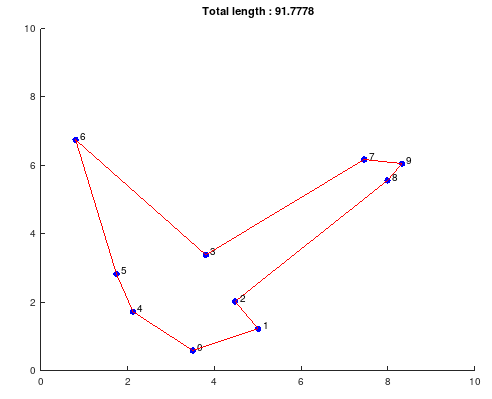
\includegraphics[width=0.8\linewidth]{img/PPI1.png}
    \caption{Chemin de l'algorithme PPI}
    \label{PPI1}
\end{figure}

\begin{figure}[!ht]
    \centering
    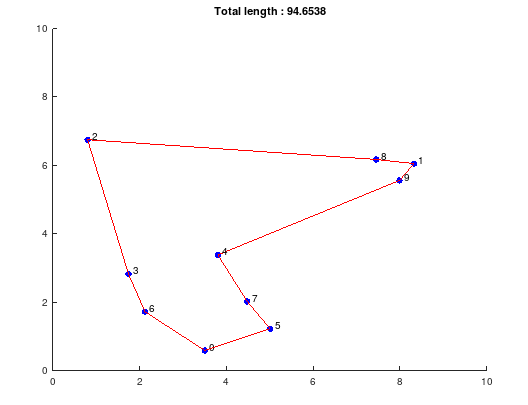
\includegraphics[width=0.8\linewidth]{img/PLI1.png}
    \caption{Chemin de l'algorithme PLI}
    \label{PLI1}
\end{figure}

\begin{figure}[!ht]
    \centering
    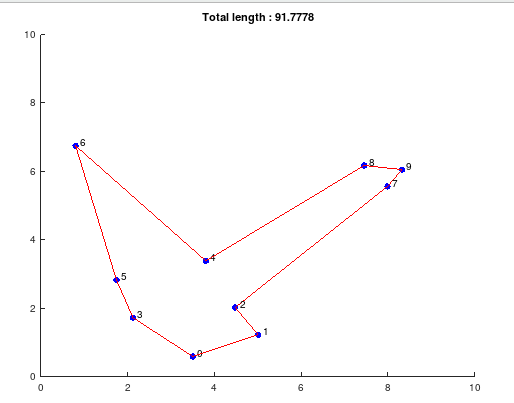
\includegraphics[width=0.8\linewidth]{img/MI1.png}
    \caption{Chemin de l'algorithme MI}
    \label{MI1}
\end{figure}

Les numéros des points correspondent à leur ordre d'ajout dans le chemin.
On voit ainsi que PPI prend bien à chaque fois le nœud le plus proche du circuit
et PLI le plus loin. On peut noter que MI donne le même résultat que PPI ici mais
on voit bien que l'ordre d'ajout est différent. Il n'est pas rare que le point de coût
d'insertion minimal et le point le plus proche du graphe coïncident : il suffit pour cela qu'on ait
un point hors circuit qui soit de distance minimal avec un point du graphe et qu'il soit suffisamment proche avec
un autre point pour avoir un coût d'insertion minimal.

On constate que, sur cet exemple, PPI et MI sont plus performants avec une longueur d'environ
92 que PLI avec une longueur de 95 mais ce n'est qu'anecdotique. En effet pour tester les algorithmes,
on doit utiliser plusieurs tests, ici 100, et plus de points, ici 50.
On obtient alors les statistiques du tableau \ref{stats}.

\begin{table}[!ht]
    \begin{center}
        \begin{tabular}{ |c|c|c|c| }
            \hline
            	Algorithme	&		PPI		    &		PLI	&		MI\\
            \hline
            Temps d'exécution moyen (ms)		&		0.3582573	&		0.2699245	&		0.2307893\\
            \hline
            Longueur moyenne		&		120.7714		&		119.7717		&		120.2111\\
            \hline
            Nombre de fois 1er		&		38	&		31	&		31\\
            \hline
            Nombre de fois 2nd		&		31	&		34		    &		35\\
            \hline
            Nombre de fois 3ème		&		31		&		35		    &		34\\
            \hline
        \end{tabular}
    \end{center}   
    \caption{Table des statistiques}
    \label{stats}    
\end{table}

On voit ainsi que les algorithmes donne des performance similaires puisque les longueurs moyennes
obtenues sont entre 119.75 et 120.8. On peut remarquer que PLI possède la meilleure performance
moyenne mais que c'est PPI qui est le plus souvent premier (38 fois sur 100). Grâce à 
l'utilisation d'un tableau de coût et d'une mise à jour intelligente ce celui-ci, le temps d'exécution
est minimale avec MI (0.23 ms) tandis qu'il est maximal avec PLI (0.36 ms) notamment
car on gère 2 tableaux et on n'effectue pas une mise à jour dynamique d'un tableau de coût d'insertion.

\clearpage

Les histogrammes des longueurs obtenus sur les figures \ref{PPI1}, \ref{PLI1} et \ref{MI1} montrent que les distributions sont assez proches de distributions normales avec des moyennes
et des écarts-types qui sont assez similaires (entre 11.8 et 12.4). Il y a juste la distribution de PLI qui semble avoir
une concentration un peu plus forte autour de 120.

\begin{figure}[!ht]
    \centering
    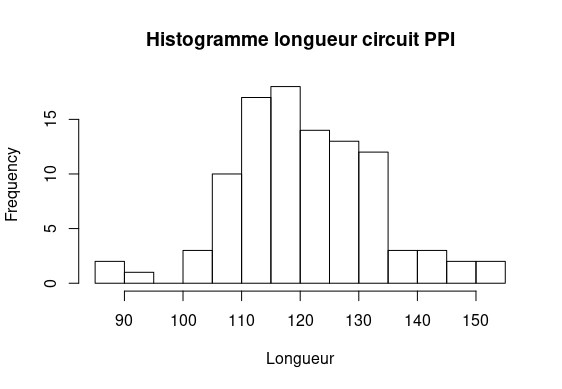
\includegraphics[width=0.8\linewidth]{img/RplotPPI.png}
    \caption{Histogramme PPI}
    \label{PPIhist}
\end{figure}

\begin{figure}[!ht]
    \centering
    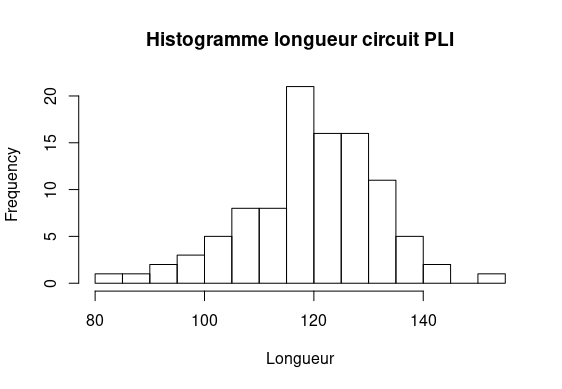
\includegraphics[width=0.8\linewidth]{img/RplotPLI.png}
    \caption{Histogramme PLI}
    \label{PLIhist}
\end{figure}

\begin{figure}[!ht]
    \centering
    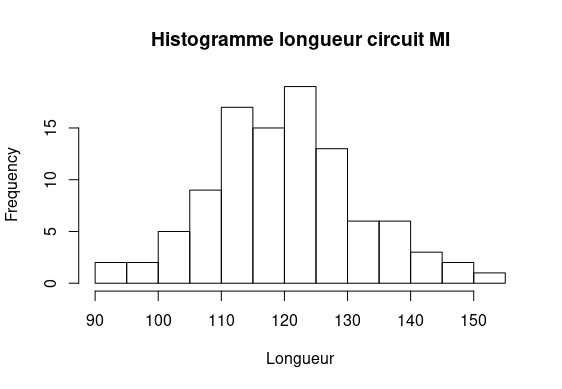
\includegraphics[width=0.8\linewidth]{img/RplotMI.png}
    \caption{Histogramme MI}
    \label{MIhist}
\end{figure}

\clearpage

\section{Annexes}

\subsection{Visualisation de tournées (plots.m)}

\lstinputlisting[language=Matlab]{plots.m}

\subsection{Visualisation de statistiques (stats.R)}
\lstinputlisting[language=R]{stats.R}
\end{document}